% Schematic report: compile with pdflatex (two runs).
\documentclass[11pt,a4paper]{article}
\usepackage[T1]{fontenc}
\usepackage[utf8]{inputenc}
\usepackage{lmodern}
\usepackage[a4paper,margin=2.2cm]{geometry}
\usepackage{microtype}
\usepackage{booktabs}
\usepackage{tabularx}
\usepackage{array}
\usepackage{amsmath}
\usepackage{xcolor}
\usepackage{tikz}
\usetikzlibrary{arrows.meta,positioning,fit,calc,backgrounds}
\usepackage{listings}
\usepackage{caption}
\usepackage{float}
\usepackage{needspace}
\usepackage{enumitem}
\usepackage{hyperref}
\hypersetup{colorlinks=true,linkcolor=black,urlcolor=black}

\setlist{nosep,leftmargin=*}
\captionsetup{font=small,labelfont=bf}
\setlength{\parskip}{3pt}
\setlength{\emergencystretch}{3em}
\renewcommand{\topfraction}{0.9}
\renewcommand{\bottomfraction}{0.8}
\renewcommand{\textfraction}{0.07}
\renewcommand{\floatpagefraction}{0.85}
\setcounter{topnumber}{3}
\setcounter{totalnumber}{5}

% Colours (RGB only)
\definecolor{llmc}{RGB}{250,222,190}
\definecolor{retc}{RGB}{205,224,247}
\definecolor{kgc}{RGB}{208,236,208}
\definecolor{datc}{RGB}{238,238,238}
\definecolor{promptc}{RGB}{255,248,214}
\definecolor{codebg}{RGB}{247,247,247}

\tikzset{
  box/.style={draw, rounded corners=2pt, align=center, font=\scriptsize, minimum height=7mm, inner sep=2.5pt},
  llm/.style={box, fill=llmc},
  ret/.style={box, fill=retc},
  kg/.style={box, fill=kgc},
  dat/.style={box, fill=datc, rounded corners=0pt},
  prm/.style={box, fill=promptc, rounded corners=0pt},
  arr/.style={-{Stealth[length=1.6mm]}, semithick},
  lab/.style={font=\tiny, midway, fill=white, inner sep=1pt},
}

\lstset{
  basicstyle=\ttfamily\scriptsize,
  breaklines=true,
  breakatwhitespace=false,
  columns=fullflexible,
  keepspaces=true,
  frame=single,
  rulecolor=\color{black!30},
  backgroundcolor=\color{codebg},
  xleftmargin=2pt, xrightmargin=2pt,
  literate={—}{{---}}1 {–}{{--}}1 {’}{{'}}1 {‘}{{`}}1 {“}{{``}}1 {”}{{''}}1 {…}{{...}}1,
}

\newcommand{\sys}[1]{\textsf{#1}}
\newcommand{\gen}{\texttt{gpt-5.4-nano}}

\title{Schematic report\\[2pt]\large Conversational QA on MultiDoc2Dial with passages and a knowledge graph}
\author{Danil Smirnov (2142049)}
\date{October 2026}


\begin{document}
\maketitle

\begin{center}
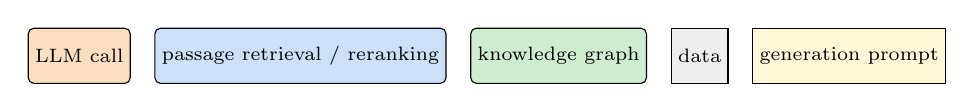
\begin{tikzpicture}[node distance=3mm]
  \node[box, fill=llmc] (a) {LLM call};
  \node[box, fill=retc, right=of a] (b) {passage retrieval / reranking};
  \node[box, fill=kgc, right=of b] (c) {knowledge graph};
  \node[box, fill=datc, rounded corners=0pt, right=of c] (d) {data};
  \node[box, fill=promptc, rounded corners=0pt, right=of d] (e) {generation prompt};
\end{tikzpicture}
\\[2pt]
{\small Colour legend used in all diagrams. The generator is always \gen{} (Azure OpenAI).}
\end{center}

% =====================================================================
\section{Data: one real conversation (Q1)}\label{sec:data}

\textbf{MultiDoc2Dial: 488 government-service documents (4,114 sections) and dialogues in which
every agent answer is grounded in the documents; about 5\% of the user questions cannot be
answered from them.}

\begin{table}[H]
\centering\footnotesize
\renewcommand{\arraystretch}{1.15}
\begin{tabularx}{\linewidth}{@{}p{1.6cm}X@{}}
\toprule
\multicolumn{2}{@{}l}{\textbf{Turn 5} (unanswerable). Gold section: \emph{Traffic Violations Bureau -- What To Do If You Receive A Traffic Ticket}}\\
\midrule
User & No. \quad (answer to the agent asking whether the ticket was issued in New York City)\\
Reference & Unfortunately, no relevant information is found.\\
LLM only & Please contact your local government office or the service provider directly [\ldots] \hfill F1 0.00\\
Best RAG & If you have a DMV Traffic Violations Bureau ticket issued in the five boroughs of New York City, you can answer most TVB tickets online [\ldots] \hfill F1 0.00\\
E & Unfortunately, no relevant information is found. \hfill F1 1.00\\
\midrule
\multicolumn{2}{@{}l}{\textbf{Turn 13}. Gold section: \emph{Traffic Violations Bureau -- APPEALS}}\\
\midrule
User & what if im a holder of a junior license?\\
Reference & you can not plead by mail or online. you still must appear for a hearing in a tvb office.\\
LLM only & If you hold a junior license, you must follow the restrictions and requirements that come with that license while driving [\ldots] \hfill F1 0.17\\
Best RAG & If you're a holder of a probationary/junior license or learner permit and you're charged with a cell phone/texting violation on or after July 1, 2013, you cannot plead by mail or online and you must appear for a hearing in a TVB office. \hfill F1 0.51\\
E & If you are a holder of a probationary/junior license or a learner permit, you cannot plead by mail or online. You must appear for a hearing in a TVB office. \hfill F1 0.67\\
\bottomrule
\end{tabularx}
\caption{Two turns of a validation dialogue, DMV domain. Best RAG is the best passage pipeline,
E the same pipeline plus graph facts.}
\label{tab:twoturns}
\end{table}

\begin{itemize}
\item Without documents the model gives generic advice; with retrieval it quotes the right rule.
\item Turn 13: E is closest to the reference because one graph fact states exactly this rule.
\item Turn 5 (``No.'') is unanswerable: the passage pipeline answers anyway, E abstains.
\end{itemize}

% =====================================================================
\section{Architectures (Q2)}\label{sec:arch}

\textbf{All systems use the same generator (\gen) and prompt; they differ only in what is put in
the context: nothing, the gold sections, retrieved passages, graph sections or facts, or passages
plus graph facts.}

\begin{figure}[H]
\centering
\textbf{(a) LLM only}\\[2pt]
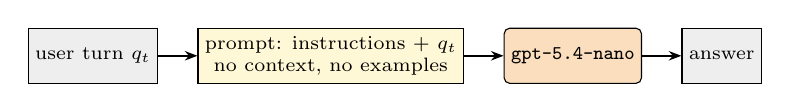
\begin{tikzpicture}[node distance=5mm]
  \node[dat] (q) {user turn $q_t$};
  \node[prm, right=of q] (p) {prompt: instructions + $q_t$\\no context, no examples};
  \node[llm, right=of p] (g) {\gen};
  \node[dat, right=of g] (a) {answer};
  \draw[arr] (q) -- (p); \draw[arr] (p) -- (g); \draw[arr] (g) -- (a);
\end{tikzpicture}

\vspace{2mm}\textbf{(b) Oracle}\\[2pt]
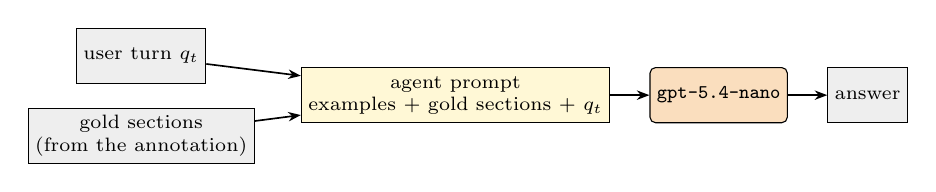
\begin{tikzpicture}[node distance=5mm]
  \node[dat] (q) {user turn $q_t$};
  \node[dat, below=3mm of q] (gs) {gold sections\\(from the annotation)};
  \node[prm, right=12mm of q, yshift=-5mm] (p) {agent prompt\\examples + gold sections + $q_t$};
  \node[llm, right=of p] (g) {\gen};
  \node[dat, right=of g] (a) {answer};
  \draw[arr] (q) -- (p); \draw[arr] (gs) -- (p); \draw[arr] (p) -- (g); \draw[arr] (g) -- (a);
\end{tikzpicture}

\vspace{2mm}\textbf{(c) Passage RAG, best pipeline (``Step 4 best'')}\\[2pt]
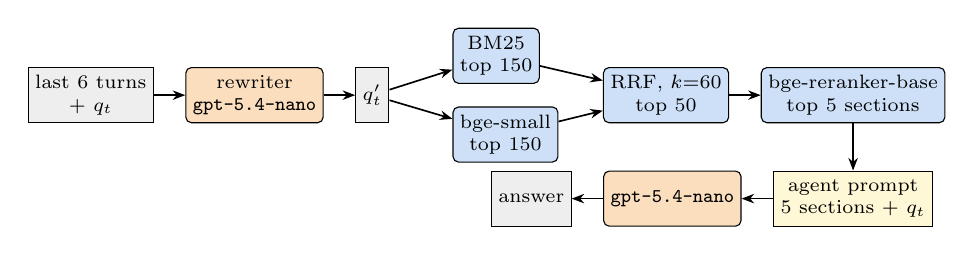
\begin{tikzpicture}[node distance=4mm]
  \node[dat] (h) {last 6 turns\\+ $q_t$};
  \node[llm, right=of h] (rw) {rewriter\\\gen};
  \node[dat, right=of rw] (qq) {$q'_t$};
  \node[ret, right=8mm of qq, yshift=5mm] (bm) {BM25\\top 150};
  \node[ret, right=8mm of qq, yshift=-5mm] (de) {bge-small\\top 150};
  \node[ret, right=8mm of bm, yshift=-5mm] (rrf) {RRF, $k{=}60$\\top 50};
  \node[ret, right=of rrf] (rr) {bge-reranker-base\\top 5 sections};
  \draw[arr] (h) -- (rw); \draw[arr] (rw) -- (qq);
  \draw[arr] (qq) -- (bm); \draw[arr] (qq) -- (de);
  \draw[arr] (bm) -- (rrf); \draw[arr] (de) -- (rrf); \draw[arr] (rrf) -- (rr);
  \node[prm, below=6mm of rr] (p) {agent prompt\\5 sections + $q_t$};
  \node[llm, left=of p] (g) {\gen};
  \node[dat, left=of g] (a) {answer};
  \draw[arr] (rr) -- (p); \draw[arr] (p) -- (g); \draw[arr] (g) -- (a);
\end{tikzpicture}

\vspace{2mm}\textbf{(d) A: graph $\to$ sections}\\[2pt]
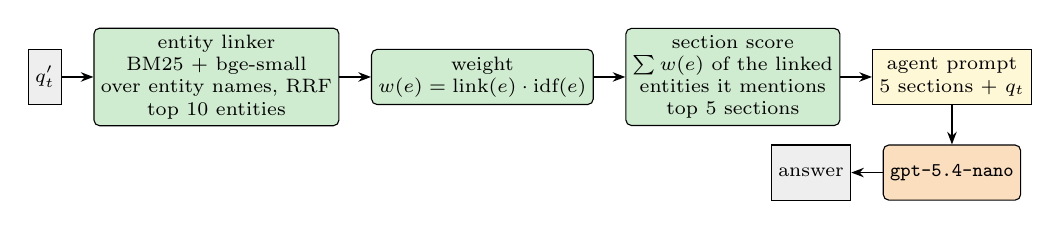
\begin{tikzpicture}[node distance=4mm]
  \node[dat] (qq) {$q'_t$};
  \node[kg, right=of qq] (lk) {entity linker\\BM25 + bge-small\\over entity names, RRF\\top 10 entities};
  \node[kg, right=of lk] (w) {weight\\$w(e)=\text{link}(e)\cdot\text{idf}(e)$};
  \node[kg, right=of w] (s) {section score\\$\sum w(e)$ of the linked\\entities it mentions\\top 5 sections};
  \node[prm, right=of s] (p) {agent prompt\\5 sections + $q_t$};
  \node[llm, below=5mm of p] (g) {\gen};
  \node[dat, left=of g] (an) {answer};
  \draw[arr] (qq) -- (lk); \draw[arr] (lk) -- (w); \draw[arr] (w) -- (s); \draw[arr] (s) -- (p); \draw[arr] (p) -- (g);
  \draw[arr] (g) -- (an);
\end{tikzpicture}

\vspace{2mm}\textbf{(e) B: graph facts only}\\[2pt]
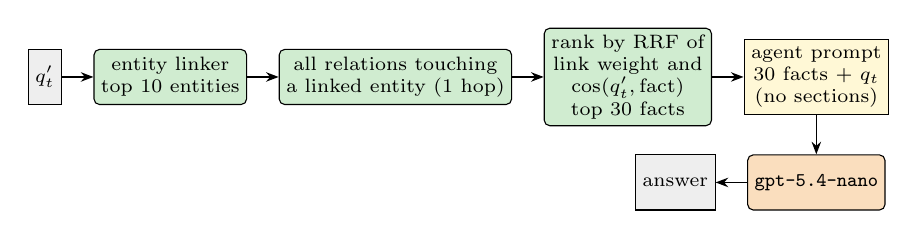
\begin{tikzpicture}[node distance=4mm]
  \node[dat] (qq) {$q'_t$};
  \node[kg, right=of qq] (lk) {entity linker\\top 10 entities};
  \node[kg, right=of lk] (adj) {all relations touching\\a linked entity (1 hop)};
  \node[kg, right=of adj] (rk) {rank by RRF of\\link weight and\\$\cos(q'_t,\text{fact})$\\top 30 facts};
  \node[prm, right=of rk] (p) {agent prompt\\30 facts + $q_t$\\(no sections)};
  \node[llm, below=5mm of p] (g) {\gen};
  \node[dat, left=of g] (an) {answer};
  \draw[arr] (g) -- (an);
  \draw[arr] (qq) -- (lk); \draw[arr] (lk) -- (adj); \draw[arr] (adj) -- (rk); \draw[arr] (rk) -- (p); \draw[arr] (p) -- (g);
\end{tikzpicture}
\caption{Architectures, part 1. All graph pipelines use the rewritten query $q'_t$ from (c).}
\label{fig:arch1}
\end{figure}

\begin{figure}[H]
\centering
\textbf{(f) C: hybrid, graph and passages fused before the reranker}\\[2pt]
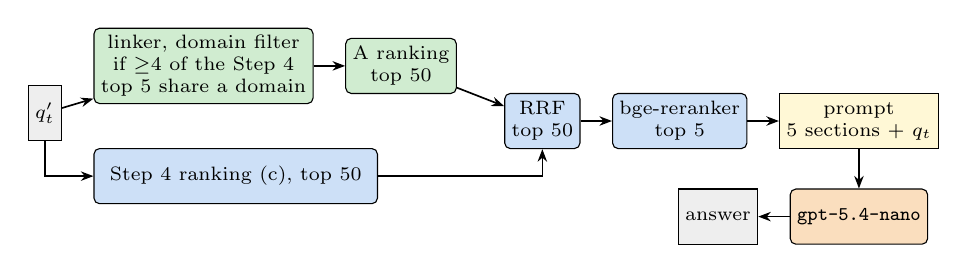
\begin{tikzpicture}[node distance=4mm]
  \node[dat] (qq) {$q'_t$};
  \node[kg, right=of qq, yshift=6mm] (lk) {linker, domain filter\\if $\ge$4 of the Step 4\\top 5 share a domain};
  \node[kg, right=of lk] (a) {A ranking\\top 50};
  \node[ret, right=of qq, yshift=-8mm, minimum width=36mm] (s4) {Step 4 ranking (c), top 50};
  \node[ret, right=6mm of a, yshift=-7mm] (rrf) {RRF\\top 50};
  \node[ret, right=of rrf] (rr) {bge-reranker\\top 5};
  \node[prm, right=of rr] (p) {prompt\\5 sections + $q_t$};
  \node[llm, below=5mm of p] (g) {\gen};
  \node[dat, left=of g] (an) {answer};
  \draw[arr] (p) -- (g); \draw[arr] (g) -- (an);
  \draw[arr] (qq) -- (lk); \draw[arr] (lk) -- (a); \draw[arr] (qq) |- (s4);
  \draw[arr] (a) -- (rrf); \draw[arr] (s4) -| (rrf); \draw[arr] (rrf) -- (rr); \draw[arr] (rr) -- (p);
\end{tikzpicture}

\vspace{2mm}\textbf{(g) D: graph as candidate generator for the reranker}\\[2pt]
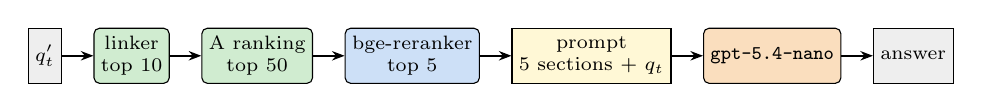
\begin{tikzpicture}[node distance=4mm]
  \node[dat] (qq) {$q'_t$};
  \node[kg, right=of qq] (lk) {linker\\top 10};
  \node[kg, right=of lk] (a) {A ranking\\top 50};
  \node[ret, right=of a] (rr) {bge-reranker\\top 5};
  \node[prm, right=of rr] (p) {prompt\\5 sections + $q_t$};
  \node[llm, right=of p] (g) {\gen};
  \node[dat, right=of g] (an) {answer};
  \draw[arr] (g) -- (an);
  \draw[arr] (qq) -- (lk); \draw[arr] (lk) -- (a); \draw[arr] (a) -- (rr); \draw[arr] (rr) -- (p); \draw[arr] (p) -- (g);
\end{tikzpicture}

\vspace{2mm}\textbf{(h) E: passages + graph facts, and the E-random control}\\[2pt]
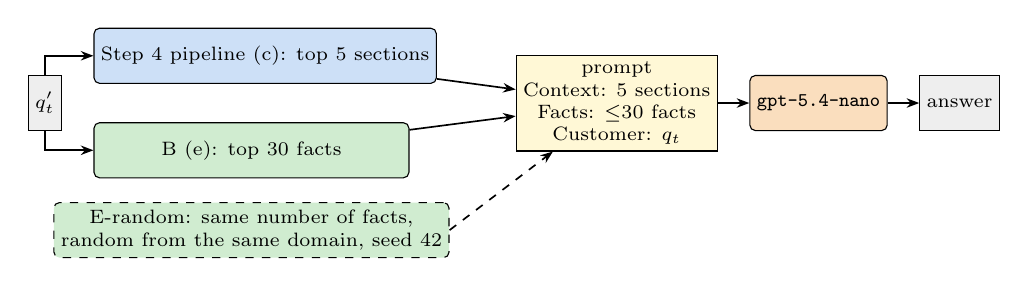
\begin{tikzpicture}[node distance=4mm]
  \node[dat] (qq) {$q'_t$};
  \node[ret, right=of qq, yshift=6mm, minimum width=40mm] (s4) {Step 4 pipeline (c): top 5 sections};
  \node[kg, right=of qq, yshift=-6mm, minimum width=40mm] (b) {B (e): top 30 facts};
  \node[kg, below=3mm of b, dashed, minimum width=40mm] (rnd) {E-random: same number of facts,\\random from the same domain, seed 42};
  \node[prm, right=10mm of s4, yshift=-6mm] (p) {prompt\\Context: 5 sections\\Facts: $\le$30 facts\\Customer: $q_t$};
  \node[llm, right=of p] (g) {\gen};
  \draw[arr] (qq) |- (s4); \draw[arr] (qq) |- (b);
  \draw[arr] (s4) -- (p); \draw[arr] (b) -- (p); \draw[arr, dashed] (rnd.east) -- (p);
  \node[dat, right=of g] (an) {answer};
  \draw[arr] (p) -- (g); \draw[arr] (g) -- (an);
\end{tikzpicture}
\caption{Architectures, part 2. C and D were tried on a 500-question development subset and
dropped; E and E-random were run on the full validation and test splits.}
\label{fig:arch2}
\end{figure}

\begin{itemize}
\item The query rewriter is the only part that sees the dialogue history; its output is used only
  for retrieval.
\item In all results except Section~\ref{sec:conv} the generator sees only the current user turn
  and the retrieved context.
\end{itemize}

% =====================================================================
\section{Graph schema (Q3)}\label{sec:schema}

\textbf{A closed schema of 9 entity types and 11 relations, stored in three layers: the document
structure, the mentions extracted by the LLM, and the resolved entities with typed relations.}

\begin{figure}[H]
\centering
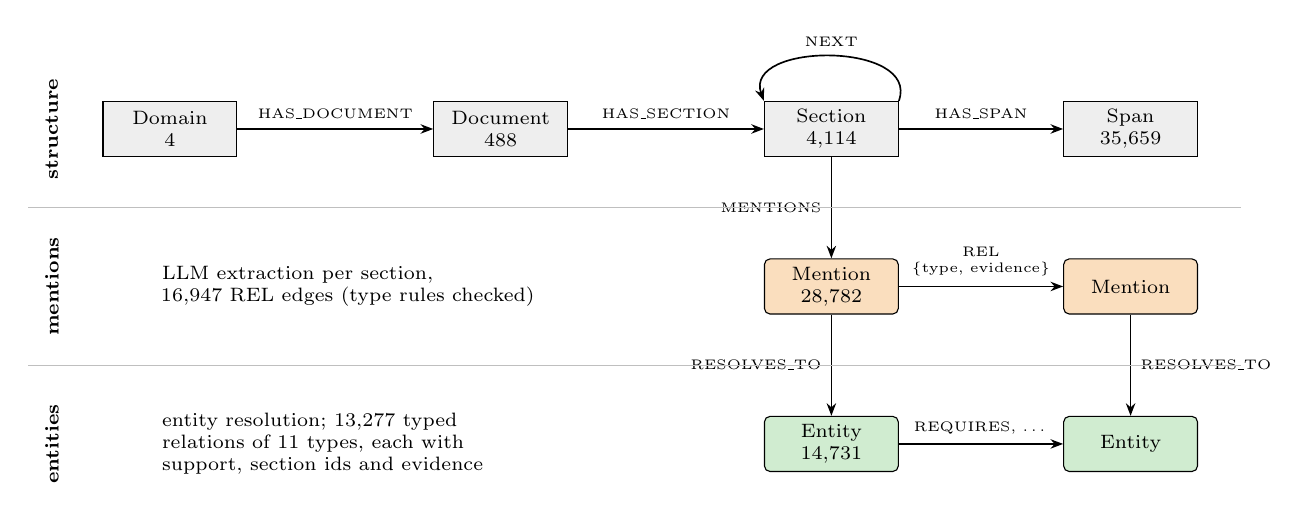
\begin{tikzpicture}
  \node[dat, minimum width=17mm] (dom) at (-0.6,0) {Domain\\4};
  \node[dat, minimum width=17mm] (doc) at (3.6,0) {Document\\488};
  \node[dat, minimum width=17mm] (sec) at (7.8,0) {Section\\4,114};
  \node[dat, minimum width=17mm] (sp) at (11.6,0) {Span\\35,659};
  \draw[arr] (dom) -- node[font=\tiny, above] {HAS\_DOCUMENT} (doc);
  \draw[arr] (doc) -- node[font=\tiny, above] {HAS\_SECTION} (sec);
  \draw[arr] (sec) -- node[font=\tiny, above] {HAS\_SPAN} (sp);
  \draw[arr] (sec.north east) to[out=70, in=110, looseness=1.2] node[font=\tiny, above] {NEXT} (sec.north west);
  \node[box, fill=llmc, minimum width=17mm] (m1) at (7.8,-2) {Mention\\28,782};
  \node[box, fill=llmc, minimum width=17mm] (m2) at (11.6,-2) {Mention};
  \draw[arr] (sec) -- node[font=\tiny, left] {MENTIONS} (m1);
  \draw[arr] (m1) -- node[font=\tiny, above, align=center] {REL\\\{type, evidence\}} (m2);
  \node[kg, minimum width=17mm] (e1) at (7.8,-4) {Entity\\14,731};
  \node[kg, minimum width=17mm] (e2) at (11.6,-4) {Entity};
  \draw[arr] (m1) -- node[font=\tiny, left] {RESOLVES\_TO} (e1);
  \draw[arr] (m2) -- node[font=\tiny, right] {RESOLVES\_TO} (e2);
  \draw[arr] (e1) -- node[font=\tiny, above] {REQUIRES, \ldots} (e2);
  \node[font=\scriptsize\bfseries, rotate=90] at (-2.1,0) {structure};
  \node[font=\scriptsize\bfseries, rotate=90] at (-2.1,-2) {mentions};
  \node[font=\scriptsize\bfseries, rotate=90] at (-2.1,-4) {entities};
  \draw[black!25] (-2.4,-1) -- (13,-1); \draw[black!25] (-2.4,-3) -- (13,-3);
  \node[font=\scriptsize, align=left, text width=5.2cm] at (1.9,-2) {LLM extraction per section,\\16,947 REL edges (type rules checked)};
  \node[font=\scriptsize, align=left, text width=5.2cm] at (1.9,-4) {entity resolution; 13,277 typed\\relations of 11 types, each with\\support, section ids and evidence};
\end{tikzpicture}
\caption{The three layers of the graph and their sizes. A retrieved section and a graph
section are the same object.}
\label{fig:layers}
\end{figure}

\begin{itemize}
\item Entity types: Service, Organization, Document, Requirement, Amount, TimeLimit, Role, Outcome,
  ContactPoint.
\item Relations: REQUIRES, PROVIDED\_BY, HAS\_AMOUNT, HAS\_TIME\_LIMIT, APPLIES\_TO, LEADS\_TO,
  EXEMPT\_FROM, DETERMINED\_BY, AVAILABLE\_AT, PART\_OF, ALTERNATIVE\_TO, each with allowed type
  pairs.
\end{itemize}

% =====================================================================
\section{How the LLM uses the graph (Q4)}\label{sec:usage}

\textbf{The LLM never calls the graph. The retriever queries it, and the LLM only sees the facts
(or sections) as text lines in its prompt.}

\begin{figure}[H]
\centering
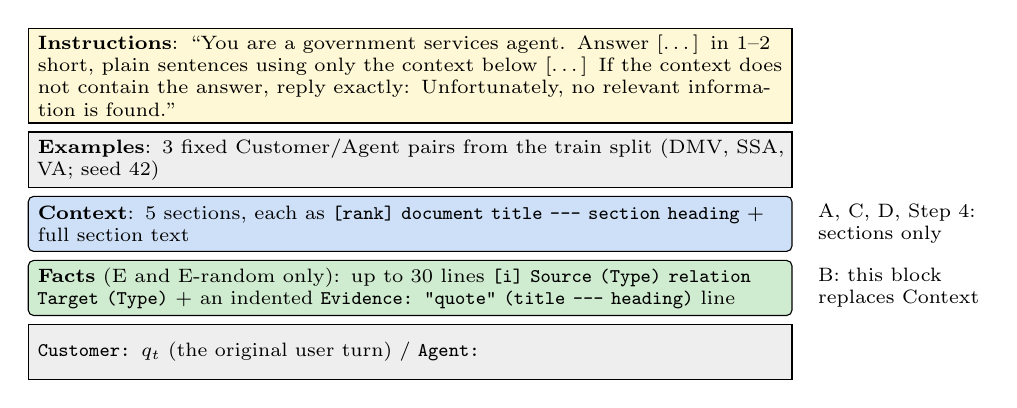
\begin{tikzpicture}[every node/.style={font=\scriptsize}]
  \node[prm, minimum width=0.8\linewidth, align=left, text width=0.78\linewidth] (i) {\textbf{Instructions}: ``You are a government services agent. Answer [\ldots] in 1--2 short, plain sentences using only the context below [\ldots] If the context does not contain the answer, reply exactly: Unfortunately, no relevant information is found.''};
  \node[dat, below=1mm of i, minimum width=0.8\linewidth, align=left, text width=0.78\linewidth] (e) {\textbf{Examples}: 3 fixed Customer/Agent pairs from the train split (DMV, SSA, VA; seed 42)};
  \node[ret, below=1mm of e, minimum width=0.8\linewidth, align=left, text width=0.78\linewidth] (c) {\textbf{Context}: 5 sections, each as \texttt{[rank] document title --- section heading} + full section text};
  \node[kg, below=1mm of c, minimum width=0.8\linewidth, align=left, text width=0.78\linewidth] (f) {\textbf{Facts} (E and E-random only): up to 30 lines \texttt{[i] Source (Type) relation Target (Type)} + an indented \texttt{Evidence: "quote" (title --- heading)} line};
  \node[dat, below=1mm of f, minimum width=0.8\linewidth, align=left, text width=0.78\linewidth] (q) {\texttt{Customer: $q_t$} (the original user turn) / \texttt{Agent:}};
  \node[right=2mm of c, align=left] {A, C, D, Step 4:\\sections only};
  \node[right=2mm of f, align=left] {B: this block\\replaces Context};
\end{tikzpicture}
\caption{Layout of the generation prompt, top to bottom. LLM only uses a shorter prompt with no
examples and no context. Average prompt length on validation: Step 4 about 6,400 characters, E
about 14,900.}
\label{fig:prompt-layout}
\end{figure}

\begin{itemize}
\item Entity linking: the rewritten query is matched to 10 entities by name (BM25 + embeddings).
\item From the entities: their sections (A), or their relations as facts, top 30 (B, E).
\end{itemize}

% =====================================================================
\section{Is the graph used as a reranker signal? (Q5)}\label{sec:rerank}

\textbf{No. The graph only changes which sections the reranker sees; no graph score enters the
ranking.}

\begin{itemize}
\item C: graph ranking and passage ranking are fused (RRF), then the cross-encoder picks the top 5
  (Figure~\ref{fig:arch2}f). D: the graph ranking alone feeds the cross-encoder.
\item Development subset: C $-0.5$ F1 (not significant), D $-1.6$; both dropped.
\item A graph score as a feature inside the ranking is a possible next experiment.
\end{itemize}

% =====================================================================
\section{What ``adding graph facts'' means (Q6)}\label{sec:facts}

\textbf{Up to 30 relations of the linked entities, one line each (triple + evidence quote +
document and section heading), in a separate Facts block after the 5 passages.}

\begin{lstlisting}[frame=none,backgroundcolor=\color{white}]
[5] probationary / junior license or learner permit (Role) exempt from plead by mail or online (Service)
    Evidence: "you cannot plead by mail or online" (Traffic Violations Bureau — APPEALS)
\end{lstlisting}

\begin{itemize}
\item 26 facts per question on average; at least one comes from a gold section in 49\% of them.
\item Control E-random: the same number of random facts from the same domain.
\end{itemize}

% =====================================================================
\section{What 4,427 counts, and how F1 is computed (Q7)}\label{sec:f1}

\textbf{4,427 = user questions (turns), not conversations; F1 is computed per question and
averaged over questions.}

\begin{itemize}
\item Validation: 661 conversations with 4--10 questions each (mean 6.7); 226 unanswerable.
\item F1: token overlap with the reference after SQuAD normalisation; an exact refusal on an
  unanswerable question scores 1.
\item EM is about 1\% for every system and not reported; SacreBLEU is not implemented.
\end{itemize}

% =====================================================================
\section{Query rewriting (Q10)}\label{sec:rewrite}

\textbf{One extra \gen{} call per follow-up turn turns the user message plus the last 6 turns
of the gold history into a self-contained search query, used only for retrieval.}

\begin{center}
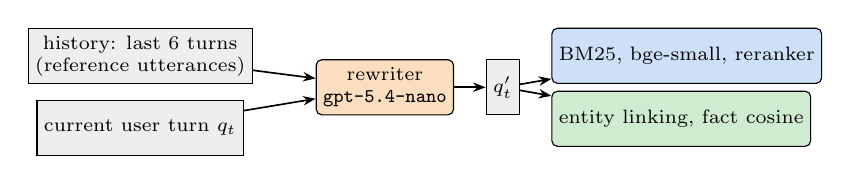
\begin{tikzpicture}[node distance=4mm]
  \node[dat] (h) {history: last 6 turns\\(reference utterances)};
  \node[dat, below=2mm of h] (q) {current user turn $q_t$};
  \node[llm, right=8mm of h, yshift=-4mm] (rw) {rewriter\\\gen};
  \node[dat, right=of rw] (qq) {$q'_t$};
  \node[ret, right=of qq, yshift=4mm] (r) {BM25, bge-small, reranker};
  \node[kg, right=of qq, yshift=-4mm] (k) {entity linking, fact cosine};
  \draw[arr] (h) -- (rw); \draw[arr] (q) -- (rw); \draw[arr] (rw) -- (qq); \draw[arr] (qq) -- (r); \draw[arr] (qq) -- (k);
\end{tikzpicture}
\end{center}

\begin{itemize}
\item Example: ``what if im a holder of a junior license?'' $\to$ ``What happens if I plead guilty
  with a junior license in TVB?''
\item First turns are not rewritten (3,767 rewrite calls for 4,427 questions).
\end{itemize}

% =====================================================================
\section{The graph retrieval step (Step 6), plainly (Q11)}\label{sec:step6}

\textbf{The question is linked to 10 graph entities, which give sections (A), facts (B), or facts
added to the normal passages (E). The graph alone is clearly worse than passages; facts added to
passages give a small gain on answerable questions that random facts do not give.}

\begin{table}[H]
\centering\small
\begin{tabular}{lccc}
\toprule
 & \multicolumn{3}{c}{F1 (\%)} \\
System & all & answerable & unanswerable \\
\midrule
LLM only & 15.8 & 15.7 & 18.4 \\
Step 4 best (passages) & 26.9 & 27.2 & 20.2 \\
A: graph sections & 23.0 & 22.4 & 32.5 \\
B: graph facts & 24.1 & 23.8 & 30.6 \\
E: passages + facts & 27.4 & 27.7 & 20.1 \\
E-random (control) & 27.4 & 27.2 & 31.9 \\
Oracle (gold sections) & 35.5 & 36.5 & 15.9 \\
\midrule
Passages, with dialogue history & 27.5 & 27.6 & 25.0 \\
Passages + facts, with dialogue history & 28.0 & 28.2 & 24.5 \\
\bottomrule
\end{tabular}
\caption{Full validation split (4,427 questions, 226 unanswerable). The last two rows use the
conversational generator of Section~\ref{sec:conv}. Test split, run once: Step 4 26.9, E 27.5,
E-random 27.3, B 23.8, LLM only 15.1, oracle 34.2; with dialogue history, passages 27.6 and
passages + facts 28.2 (Section~\ref{sec:graphrag}).}
\label{tab:main}
\end{table}

\begin{itemize}
\item Evaluated by linking recall (66.5\%), section Recall@5, F1 with paired bootstrap, the
  random-facts control, answerable and unanswerable separately.
\item E vs Step 4: $+0.5$ F1 on answerable questions; E vs E-random: $+0.6$.
\end{itemize}

% =====================================================================
\section{Cost (Q12)}\label{sec:cost}

\textbf{The whole project cost EUR 34.56 on Azure (164.6\,M input and 11.6\,M output tokens).
Per 1,000 conversations: about EUR 2 for Step 4 and EUR 3.5--4.4 for E.}

\begin{itemize}
\item These per-turn numbers are estimated from the stored prompts and answers; usage is now
  recorded per call (input, cached input, output, reasoning tokens), and the measured numbers are
  in Section~\ref{sec:models}.
\item Building the graph once cost about EUR 5--7.
\end{itemize}

% =====================================================================
\section{Conversational generator (new experiment)}\label{sec:conv}

\textbf{Giving the generator the whole conversation (G2) helps on answerable questions ($+0.8$ F1)
but halves abstention. Taking the abstain decision from the current prompt (G2 + abstain(G0))
gives the best overall F1 ($+0.6$ to $+0.7$), at twice the input tokens.}

\begin{itemize}
\item The rewritten query in the prompt (G1, G3) makes results worse.
\item Cheaper abstention decisions both lose: a yes/no classifier call ($-1.3$ / $-1.0$) and a
  reranker-score threshold ($-0.6$).
\end{itemize}

% =====================================================================
\section{Generator models (Q12, new experiment)}\label{sec:models}

\textbf{gpt-5.4-nano stays the generator. gpt-5-nano and gpt-6-luna answer as well when they
answer, but refuse more answerable questions, so they are 1.0--1.8 F1 worse on them; gpt-5-nano
spends many hidden reasoning tokens, and gpt-6-luna is the cheapest.}

\begin{table}[H]
\centering\footnotesize
\begin{tabular}{llccccc}
\toprule
 & & \multicolumn{2}{c}{F1} & $\Delta$ answerable & abstain recall / & USD per 1,000 \\
 & Model & all & answerable & vs gpt-5.4-nano & false abstention & conversations \\
\midrule
Passages & gpt-5.4-nano & 27.6 & 27.6 & -- & 27.4 / \phantom{0}5.7 & 3.91 \\
 & gpt-5-nano & 27.6 & 26.5 & $-1.0$ [$-1.4$, $-0.6$] & 46.0 / 12.5 & 4.95 \\
 & gpt-6-luna & 26.8 & 25.8 & $-1.8$ [$-2.2$, $-1.3$] & 45.6 / 17.3 & 1.96 \\
\midrule
Passages & gpt-5.4-nano & 28.1 & 28.4 & -- & 22.6 / \phantom{0}3.9 & 7.30 \\
+ facts & gpt-5-nano & 28.1 & 26.8 & $-1.6$ [$-2.0$, $-1.2$] & 51.3 / 11.6 & 5.94 \\
 & gpt-6-luna & 27.3 & 26.6 & $-1.8$ [$-2.2$, $-1.4$] & 40.3 / 14.2 & 3.89 \\
\bottomrule
\end{tabular}
\caption{Generator models on validation, with dialogue history and the abstention decision of
Section~\ref{sec:conv}; only the generator changes model, all three run fresh with usage logging.
$\Delta$: paired bootstrap difference on answerable questions. On all questions gpt-5-nano ties
($-0.0$) and gpt-6-luna loses 0.8 in both pipelines. Cost at USD list prices (Azure Retail Prices
API, Global Standard, East US 2, 21 October 2026; the deployment type is not confirmed).}
\label{tab:models}
\end{table}

\begin{table}[H]
\centering\footnotesize
\begin{tabular}{lccccc}
\toprule
Passages + facts & answered & F1 on & mean & F1, questions & tokens / turn \\
 & (of 4,201) & own answers & words & all three answer & in / out (reasoning) \\
\midrule
gpt-5.4-nano & 4,036 & 29.5 & 46.4 & 30.8 & 5,793 / 106 (0) \\
gpt-5-nano & 3,712 & 30.1 & 40.3 & 30.7 & 5,532 / 1,578 (1,435) \\
gpt-6-luna & 3,603 & 30.6 & 34.3 & 30.8 & 5,511 / 176 (102) \\
\bottomrule
\end{tabular}
\caption{Answerable questions only. On the 3,443 questions all three models answer, F1 is the
same (gpt-5-nano $-0.1$ [$-0.5$, 0.2], gpt-6-luna $-0.0$ [$-0.4$, 0.4]); with passages only the
same holds (30.7, 31.0, 31.1 on 3,326 questions). Tokens: recorded usage of the generator calls.}
\label{tab:models2}
\end{table}

\begin{itemize}
\item The loss comes from refusals, not from worse answers: the newer models answer 83--88\% of
  the answerable questions, gpt-5.4-nano 94--96\%, and write shorter answers.
\item gpt-5-nano spends about 1,400 hidden reasoning tokens per turn, so its low price per token
  does not make it cheaper; gpt-6-luna costs about half as much as gpt-5.4-nano.
\item Refusal decision from gpt-5.4-nano with the answer of a newer model: no significant gain
  ($-0.3$ to $+0.2$ F1).
\end{itemize}

% =====================================================================
\section{When does the graph help? (Q14)}\label{sec:graphhelp}

\textbf{Mostly where passage retrieval misses the answer but a graph fact still comes from the
right section. A cheap router cannot find these questions before generation, so always adding the
facts stays the best choice.}

\begin{table}[H]
\centering\small
\begin{tabular}{lrccc}
\toprule
Questions (validation, with dialogue history) & $n$ & Passages & + graph facts & $d$ [95\% CI] \\
\midrule
All & 4,427 & 27.5 & 28.0 & $+0.5$ [0.1, 0.9] \\
Passages miss, a fact from the gold section & 342 & 20.6 & 25.2 & $+4.6$ [2.7, 6.6] \\
Passages hit, no fact from the gold section & 1,005 & 31.9 & 30.9 & $-1.0$ [$-1.9$, $-0.1$] \\
Follow-up turns & 3,767 & 27.6 & 28.2 & $+0.6$ [0.1, 1.1] \\
First turns & 660 & 26.6 & 26.6 & $-0.0$ [$-0.6$, 0.7] \\
\bottomrule
\end{tabular}
\caption{F1 of passages and passages + graph facts by question type; $d$ is the paired difference.}
\label{tab:graphhelp}
\end{table}

\begin{itemize}
\item An oracle choosing the better configuration per question gains 3.3 F1, but the better of two
  runs of the same system already gains 2.9: the oracle gain is mostly run-to-run noise.
\item A router on signals available before generation (reranker scores, fact overlap, dialogue
  position) picks the better configuration only 52\% of the time and is 0.5 F1 worse than always
  adding the facts.
\end{itemize}

% =====================================================================
\section{Graph RAG variants (Step 7)}\label{sec:graphrag}

\textbf{Appending the one-hop facts stays the best use of the graph. Keeping only the 10 facts
with the best cross-encoder score cuts the generator input by a third but is slightly worse on test; using the
graph to rerank sections lowers recall.}

\begin{table}[H]
\centering\small
\begin{tabular}{lcccc}
\toprule
 & \multicolumn{2}{c}{Validation} & \multicolumn{2}{c}{Test (run once)} \\
System (with dialogue history) & F1 all & answerable & F1 all & answerable \\
\midrule
Passages & 27.5 & 27.6 & 27.6 & 27.5 \\
Passages + 30 facts & 28.0 & 28.2 & 28.2 & 28.4 \\
Passages + top 10 facts & 28.0 & 28.3 & 27.8 & 28.1 \\
\bottomrule
\end{tabular}
\caption{Final systems. Top 10 facts: scored with the cross-encoder of the passage pipeline;
35--36\% fewer generator input tokens than 30 facts. Test: 30 facts $+0.6$ over passages
[0.1, 1.0]; top 10 facts $-0.4$ against 30 facts [$-0.7$, 0.0].}
\label{tab:graphrag}
\end{table}

\begin{itemize}
\item The cross-encoder filter drops the facts from other sections that recover retrieval misses;
  putting those first recovers them, without an overall gain.
\item Graph score added to the cross-encoder: R@5 falls for every weight above 0 (67.8 to 54.6 on
  dev-500), so no generation run. Two-hop paths reach no gold section that one-hop facts miss.
\end{itemize}

% =====================================================================
\section{Sources per answer (Q13)}\label{sec:sources}

\textbf{Every answer can show the sections it is based on. Asked to cite the passages and facts it
used, the model names a gold section first in 42\% of the answered questions, at no cost in F1;
the limit is retrieval, not the citations.}

\begin{table}[H]
\centering\small
\begin{tabular}{lccc}
\toprule
Answered questions (validation) & all & gold section in top 5 & gold not retrieved \\
\midrule
Post-hoc: highest answer overlap is gold & 39.5\% & 59.7\% & 1.4\% \\
Model citation: first cited source is gold & 42.2\% & 63.4\% & 2.6\% \\
Gold section anywhere in the prompt & 73.2\% & 100\% & 22.6\% \\
\bottomrule
\end{tabular}
\caption{Passages + 30 facts with dialogue history (unchanged system), 4,181--4,189 answered
questions. Post-hoc: the passage or fact section whose prompt text shares the most answer
tokens, no LLM calls. Model citation: the generator ends its answer with [2] or [F7]; each fact
maps to the section of its evidence quote.}
\label{tab:sources}
\end{table}

\begin{itemize}
\item Citations cost no quality: F1 $+0.3$ [0.0, 0.6] with the citations stripped, false abstention
  4.4\% against 4.6\%, about 56 extra tokens per answer (50 input, 6 output).
\item 1.8 sections are cited per answer; 0.9\% of the answers cite nothing and 1.8\% contain a number
  that is not in the prompt.
\end{itemize}

% =====================================================================
\section{Agents: sufficiency check and tool use}\label{sec:agents}

\textbf{The model can tell when the retrieved context lacks the gold section, but neither a second
search nor a tool-calling agent recovers it often enough to pay off; an agent that refuses on its own
almost never refuses.}

\begin{table}[H]
\centering\small
\begin{tabular}{lccc}
\toprule
dev-500, against E with citations & $\Delta$ F1 all & $\Delta$ answerable & USD / 1,000 turns \\
\midrule
E: passages + 30 facts & --- & --- & 1.39 \\
A1: check + one extra round, abstain(G0) & $-0.6$ [$-1.6$, 0.4] & $+0.1$ [$-0.5$, 0.6] & 2.29 ($+65\%$) \\
A2: tools, abstain(G0) & $-1.5$ [$-2.9$, $-0.1$] & $-0.9$ [$-2.0$, 0.1] & 1.98 ($+42\%$) \\
A2: tools, own refusal & $-2.8$ [$-4.5$, $-1.3$] & $-0.5$ [$-1.6$, 0.6] & 1.23 ($-12\%$) \\
\bottomrule
\end{tabular}
\caption{500 questions, 31 unanswerable. Paired bootstrap differences to E (passages + 30 facts,
G2 + abstain(G0), citations). Rule fixed in advance: keep a variant only if the interval on all
questions is above 0, or it ties E at 10\% lower cost; no variant qualified, so none was run on the
full validation or the test split.}
\label{tab:agents}
\end{table}

\begin{itemize}
\item \textbf{A1, fixed controller.} One call checks (query, top 5 sections, facts) and says whether they suffice.
  If not, one extra round: a new query from what is missing, retrieval and reranking again, facts of
  the newly linked entities, then answer or refuse. The check works (Youden's $J$ 0.33 [0.23, 0.42]
  against ``gold section in context''; it says insufficient on 58\% of the unanswerable questions), and
  46\% of the questions take the round. But the new query alone finds a gold section less often than
  E's query (45.5\% against 53.5\%), the union raises passage recall by only 5.6 points, and the larger
  context makes G0 abstain less (abstain recall 32\% against 42\%). Refusing when a second check is
  still insufficient is worse ($-6.6$).
\item \textbf{A2, tool-calling agent.} It starts from E's context and may call a passage search or a fact
  lookup up to 3 times. It used a tool on 44\% of the questions (none reached the limit). With its own
  refusal it ties E on answerable questions at 12\% lower cost, but refuses almost never (abstain recall 3\%),
  hence $-2.8$ overall.
\item \textbf{Exploratory, not in the plan:} on the 213 answerable questions of A1's extra round, a gold section is
  at ranks 6--10 of E's own reranked list for 8.9\% of them, against 5.6\% from the new query
  (12.7\% together). Listed as future work, since it was chosen after seeing the result.
\end{itemize}

% =====================================================================
\section{LLM judge}\label{sec:judge}

\textbf{A second model scores the answers of the final systems as correct, partial or incorrect. It agrees
with hand labels well enough ($\kappa$ 0.65) and confirms the test ranking of token F1 more clearly:
passages + 30 facts are best, and keeping only the top 10 facts costs quality.}

\begin{table}[H]
\centering\small\setlength{\tabcolsep}{4pt}
\begin{tabular}{lcccc}
\toprule
 & \multicolumn{2}{c}{Validation (4,427)} & \multicolumn{2}{c}{Test (4,334)} \\
System (with dialogue history) & judge & F1 & judge & F1 \\
\midrule
P: passages & 66.3 & 27.5 & 67.3 & 27.6 \\
E: passages + 30 facts & 66.7 & 28.0 & 68.5 & 28.2 \\
V1: passages + top 10 facts & 66.9 & 28.0 & 67.3 & 27.8 \\
\midrule
E vs P & $+0.4$ [$-0.4$, 1.3] & $+0.5$ [0.1, 0.9] & $+1.3$ [0.3, 2.2] & $+0.6$ [0.2, 1.0] \\
V1 vs E & $+0.2$ [$-0.6$, 1.0] & $-0.0$ [$-0.4$, 0.4] & $-1.2$ [$-2.0$, $-0.4$] & $-0.4$ [$-0.7$, 0.0] \\
\bottomrule
\end{tabular}
\caption{Judge score: correct = 1, partial = 0.5, incorrect = 0; abstentions scored by rule (correct only on
unanswerable turns), citations stripped. Differences are paired bootstrap intervals on the same questions.
Evaluation only: no system was re-selected on the judge.}
\label{tab:judge}
\end{table}

\begin{itemize}
\item \textbf{Setup.} gpt-6-luna sees the last four turns, the question, the reference, the gold section and the
  context given to the generator, and rates the answer; separately it says whether the answer is supported.
  USD 7.8 for validation and test together.
\item \textbf{Human check.} 60 answers of P, E and V1, half at random and half where judge and F1 disagree most,
  labelled by hand with the verdict hidden: $\kappa$ 0.65 for the three classes (0.66 on the random half, 0.59
  on the disagreement half), 0.69 for correct vs not, 90\% agreement ($\kappa$ 0.75) on correct+partial vs
  incorrect.
\item \textbf{Caveats.} Judge and generator are from the same model family. The judge is stricter than the
  human labels (in 9 of the 12 disagreements its verdict is lower). One test question is left out for all
  three systems because the content filter blocked the judge prompt. On dev-500 the agents were scored too, but
  their extended contexts are not stored, so their ``supported'' is checked against the gold section only.
\end{itemize}

% =====================================================================
\section*{Open items (Planned)}
\begin{itemize}
\item Q9, extraction precision with entities and relations evaluated separately on documents
  annotated by hand.
\end{itemize}


\end{document}
